% !TeX root = ../dissertation.tex
\chapter{Implementation}

\section{Architectual Overview}


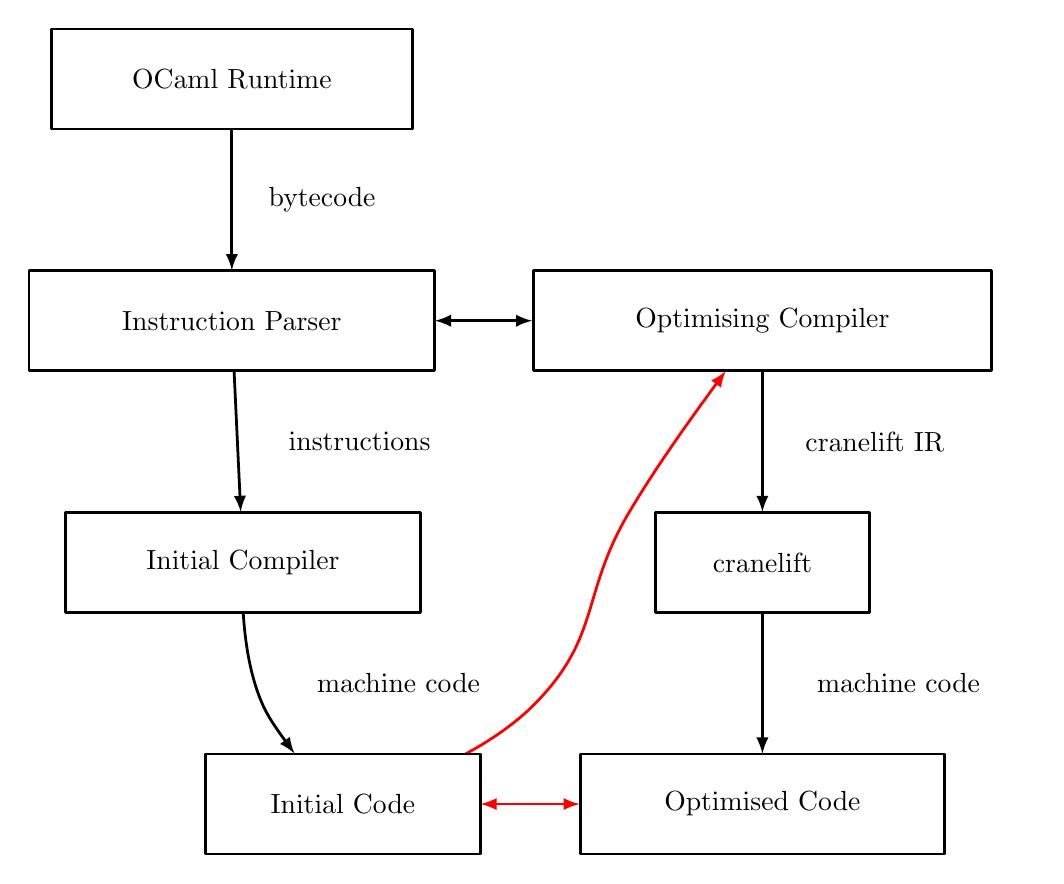
\begin{tikzpicture}[>=latex,line join=bevel,]
  \pgfsetlinewidth{1bp}
%%
\begin{scope}
  \pgfsetstrokecolor{black}
  \definecolor{strokecol}{rgb}{1.0,1.0,1.0};
  \pgfsetstrokecolor{strokecol}
  \definecolor{fillcol}{rgb}{1.0,1.0,1.0};
  \pgfsetfillcolor{fillcol}
  \filldraw (0.0bp,0.0bp) -- (0.0bp,297.0bp) -- (362.0bp,297.0bp) -- (362.0bp,0.0bp) -- cycle;
\end{scope}
\begin{scope}
  \pgfsetstrokecolor{black}
  \definecolor{strokecol}{rgb}{1.0,1.0,1.0};
  \pgfsetstrokecolor{strokecol}
  \definecolor{fillcol}{rgb}{1.0,1.0,1.0};
  \pgfsetfillcolor{fillcol}
  \filldraw (0.0bp,0.0bp) -- (0.0bp,297.0bp) -- (362.0bp,297.0bp) -- (362.0bp,0.0bp) -- cycle;
\end{scope}
\begin{scope}
  \pgfsetstrokecolor{black}
  \definecolor{strokecol}{rgb}{1.0,1.0,1.0};
  \pgfsetstrokecolor{strokecol}
  \definecolor{fillcol}{rgb}{1.0,1.0,1.0};
  \pgfsetfillcolor{fillcol}
  \filldraw (0.0bp,0.0bp) -- (0.0bp,297.0bp) -- (362.0bp,297.0bp) -- (362.0bp,0.0bp) -- cycle;
\end{scope}
  \pgfsetcolor{black}
  % Edge: ocaml_runtime -> instruction_parser
  \draw [->] (73.0bp,260.8bp) .. controls (73.0bp,249.16bp) and (73.0bp,233.55bp)  .. (73.0bp,210.18bp);
  \definecolor{strokecol}{rgb}{0.0,0.0,0.0};
  \pgfsetstrokecolor{strokecol}
  \draw (105.5bp,235.5bp) node {bytecode};
  % Edge: instruction_parser -> optimising_compiler
  \draw [<->] (146.12bp,192.0bp) .. controls (161.16bp,192.0bp) and (166.08bp,192.0bp)  .. (181.11bp,192.0bp);
  % Edge: instruction_parser -> initial_compiler
  \draw [->] (73.809bp,173.8bp) .. controls (74.357bp,162.16bp) and (75.092bp,146.55bp)  .. (76.192bp,123.18bp);
  \draw (119.0bp,148.5bp) node {instructions};
  % Edge: optimising_compiler -> cranelift
  \draw [->] (264.0bp,173.8bp) .. controls (264.0bp,162.16bp) and (264.0bp,146.55bp)  .. (264.0bp,123.18bp);
  \draw (304.5bp,148.5bp) node {cranelift IR};
  % Edge: cranelift -> optimised_code
  \draw [->] (264.0bp,86.799bp) .. controls (264.0bp,75.163bp) and (264.0bp,59.548bp)  .. (264.0bp,36.175bp);
  \draw (313.0bp,61.5bp) node {machine code};
  % Edge: initial_compiler -> compiled_code
  \draw [->] (77.103bp,86.699bp) .. controls (77.721bp,76.765bp) and (79.471bp,64.265bp)  .. (84.0bp,54.0bp) .. controls (85.445bp,50.724bp) and (87.289bp,47.51bp)  .. (95.546bp,36.228bp);
  \draw (133.0bp,61.5bp) node {machine code};
  % Edge: compiled_code -> optimising_compiler
  \pgfsetcolor{red}
  \draw [->] (157.08bp,36.003bp) .. controls (166.06bp,40.865bp) and (174.92bp,46.835bp)  .. (182.0bp,54.0bp) .. controls (206.03bp,78.314bp) and (198.53bp,93.611bp)  .. (216.0bp,123.0bp) .. controls (224.7bp,137.63bp) and (235.56bp,153.2bp)  .. (250.79bp,173.89bp);
  % Edge: compiled_code -> optimised_code
  \draw [<->] (162.55bp,18.0bp) .. controls (177.79bp,18.0bp) and (182.99bp,18.0bp)  .. (198.21bp,18.0bp);
  % Node: instruction_parser
\begin{scope}
  \definecolor{strokecol}{rgb}{0.0,0.0,0.0};
  \pgfsetstrokecolor{strokecol}
  \draw (146.0bp,210.0bp) -- (0.0bp,210.0bp) -- (0.0bp,174.0bp) -- (146.0bp,174.0bp) -- cycle;
  \draw (73.0bp,192.0bp) node {Instruction Parser};
\end{scope}
  % Node: optimising_compiler
\begin{scope}
  \definecolor{strokecol}{rgb}{0.0,0.0,0.0};
  \pgfsetstrokecolor{strokecol}
  \draw (346.5bp,210.0bp) -- (181.5bp,210.0bp) -- (181.5bp,174.0bp) -- (346.5bp,174.0bp) -- cycle;
  \draw (264.0bp,192.0bp) node {Optimising Compiler};
\end{scope}
  % Node: cranelift
\begin{scope}
  \definecolor{strokecol}{rgb}{0.0,0.0,0.0};
  \pgfsetstrokecolor{strokecol}
  \draw (302.5bp,123.0bp) -- (225.5bp,123.0bp) -- (225.5bp,87.0bp) -- (302.5bp,87.0bp) -- cycle;
  \draw (264.0bp,105.0bp) node {cranelift};
\end{scope}
  % Node: initial_compiler
\begin{scope}
  \definecolor{strokecol}{rgb}{0.0,0.0,0.0};
  \pgfsetstrokecolor{strokecol}
  \draw (141.0bp,123.0bp) -- (13.0bp,123.0bp) -- (13.0bp,87.0bp) -- (141.0bp,87.0bp) -- cycle;
  \draw (77.0bp,105.0bp) node {Initial Compiler};
\end{scope}
  % Node: compiled_code
\begin{scope}
  \definecolor{strokecol}{rgb}{0.0,0.0,0.0};
  \pgfsetstrokecolor{strokecol}
  \draw (162.5bp,36.0bp) -- (63.5bp,36.0bp) -- (63.5bp,0.0bp) -- (162.5bp,0.0bp) -- cycle;
  \draw (113.0bp,18.0bp) node {Initial Code};
\end{scope}
  % Node: optimised_code
\begin{scope}
  \definecolor{strokecol}{rgb}{0.0,0.0,0.0};
  \pgfsetstrokecolor{strokecol}
  \draw (329.5bp,36.0bp) -- (198.5bp,36.0bp) -- (198.5bp,0.0bp) -- (329.5bp,0.0bp) -- cycle;
  \draw (264.0bp,18.0bp) node {Optimised Code};
\end{scope}
  % Node: ocaml_runtime
\begin{scope}
  \definecolor{strokecol}{rgb}{0.0,0.0,0.0};
  \pgfsetstrokecolor{strokecol}
  \draw (138.0bp,297.0bp) -- (8.0bp,297.0bp) -- (8.0bp,261.0bp) -- (138.0bp,261.0bp) -- cycle;
  \draw (73.0bp,279.0bp) node {OCaml Runtime};
\end{scope}
%
\end{tikzpicture}



I have implemented a Rust static library which is linked in to the OCaml runtime library and
\texttt{ocamlrun} (the interpreter).
\texttt{ocamlrun} hooks into this library when it loads bytecode and when it starts
interpreting it.
If the JIT is enabled (either by setting an environment variable or enabling it by default at
compile time),
when the bytecode load hook is run the \textbf{initial compiler} will execute.

The initial compiler parses the bytecode into a stream of instructions and for each bytecode
instruction
it emits assembly with the same semantics to a buffer. After all code has been emitted (including
headers
and footers with shared routines) relocations are performed and the buffer is marked as executable.

When \texttt{ocamlrun} then calls the hook to start interpretation, the library instead jumps to
this assembly code which then performs the same operations as the interpreter - except that every
instruction has effectively been inlined.

When an OCaml closure is applied\footnote{all non-primitive function calls are translated to
    closure application}
a closure execution count is incremented. Once this count passes a configurable threshold the code
instead
branches in to the \textbf{optimising compiler}.

The optimising compiler operates on the level of a single function. It starts by doing a
depth-first search to discover all the basic blocks in the function. It then iterates over this
again producing Cranelift IR Format (CLIF) which is passed to the machinery of
\textbf{cranelift}. The CLIF code produced abstracts away the use of the stack allowing cranelift
to perform its register allocation. The function's code pointer is updated and any future calls
(including the originally triggering call) will use the optimised implementation.

\section{The initial compiler}

There were two milestones in the project where the initial compiler was complete: after the
implementation of the initial compiler and after the integration with the optimising compiler. The
essential difference between them is the addition of a level of pointer indirection at function
calls to allow patching the address of a function after it has been optimised.

I will describe the first implementation in this section and describe the modifications made to
support dynamic recompilation in the subsequent section REF.

\subsection{Overview of design}

In order to ensure correctness, the initial compiler produces assembly with \emph{exactly the same
    semantics} as the interpreter does (with minor exceptions covered later). The exact same
operations
are performed in the same order as the bytecode running in the interpreter performs.

The only difference is rather than use bytecode, the operations are inlined into direct assembly.
Bytecode branches are translated to machine code branches. There are two reasons why it is
reasonable to expect this to be faster:

\begin{enumerate}
    \item This design integrates much better into the instruction pipelines, branch prediction and
          out-of-order execution modern CPUs are capable of
    \item Operands can be hard-coded into the machine code rather than requiring another memory
          lookup. For example, rather than performing generalised pointer addition when looking up
          a field
          the exact offset can be included in the addressing mode.
\end{enumerate}

\subsection{Main library used}

The project makes use of the \texttt{dynasm-rs} library. The design of this library allows for
writing assembly code snippets in the source code. The assembly is validated and mostly assembled
at compile time using Rust procedural macros and a much smaller runtime library deals with any
relocations and labels.

This library was a great success as it allowed me to operate at the level of the library without
being concerned about how the assembly maps to binary. The ahead-of-time aspects means there was
very little overhead at runtime - much less than alternative approaches like making an assembly
builder or printing assembly and forking out to an assembler would use.

\subsection{Mapping of the abstract machine}

The first compiler uses a fairly direct translation from OCaml bytecode to assembly.

The x86\_64 registers \texttt{r12-r15} (callee-saved in the System V calling convention) are used
to store the OCaml registers - however the system PC is used instead of the bytecode pointer.

\subsection{Implementation overview}

The compiler is triggered on the first time a `section' is loaded - for normal programs this is at
startup and for programs using the OCaml toplevel REPL this is after every statement is typed.

The compiler first emits a standard function header entrypoint which saves callee-saved registers
used by the compiler and aligns the C stack. A longjmp handler is set up for exceptions and then
for each bytecode instruction assembly with the same semantics is emitted.

During this process \texttt{dynasm-rs} dynamic labels are used to set up relocations: these
labels are defined before every bytecode instruction and can be referenced by any other
instruction. DynASM translates these at runtime into pc-relative jumps.

After all instructions are done, some shared code used by the instructions is emitted.
\texttt{dynasm-rs} then performs relocations and uses \texttt{mmap} to mark the region of code as
executable.

The overall signature of the assembly produced by this process is a single function taking no
arguments and returning an OCaml value. OCaml closure applications (function calls) do not produce
a stack frame on the C stack - the existing machinery using the OCaml stack is used instead.

The main code of the compiler itself is contained in a 2000 line file
(\texttt{src/rust/ocaml-jit-staticlib/src/compiler/emit\_code.rs}). Most of this is taken up by a
Rust large pattern match for each of the bytecode instructions. As a very simple example of what
the code looks like consider the implemenation of the \texttt{Add} instruction. It adds the value
at the top of the OCaml stack to the accumulator and stores the result in the accumulator. Note
that the OCaml integer format means a decrement is required. In the original assembler it is
implemented as so:

\inputminted{c}{snippets/add.c}

In the compiler the case is instead:

\inputminted{rust}{snippets/add.rs}

which has exactly the same semantics. Note \texttt{r\_accu} and \texttt{r\_sp}
are aliases for \texttt{r13} and \texttt{r15}.

I repeated this process for every bytecode instruction. More involved instructions call into
OCaml runtime or custom-written C functions - the state of the registers is pushed to the stack
and interpreted as a struct by the calling functions.

\subsection{Further details}

The above explanation is an over-simplification. Here is an non-exhaustive list of complicating
factors:

\begin{itemize}
    \item There is extensive optional support to support tracing instructions and events (described
          in section \ref{tracing})
    \item Callbacks from C to OCaml code require special handling
    \item The compiler returns a pointer to the first instruction to support OCaml's
          metaprogramming \texttt{ocaml\_reify\_bytecode} program used in the implementation of
          things like the
          toplevel \texttt{ocaml} program.
    \item Function application is a fairly involved process and there are checks to resize the
          stack and check for signals as well as the fundamental complexity of the push-enter
          model.
    \item Registers need to be saved and restored at safepoints to allow the garbage collector to
          use them
    \item Certain operations are involved enough that instead of inline the definition in
          hand-written assembly, I push the registers to the C stack and call a C primitive to
          implement the
          operation (taking the registers as a struct)
    \item The compiler stores a persistent data structure of the sections to allow mapping bytecode
          addresses to
          machine code addresses and allow for cleanup after a section is freed.
\end{itemize}

Some of these are covered later but for some I will only mention them here to note their existence
- the actual details are in the code.

\subsection{Implementation strategy}

Implementation followed an incremental and highly test-driven strategy over multiple weeks. The
initial focus was on building a system sophisticated enough to run a hello world program
implementing the bare minimum instructions to support this.

I then slowly expanded the complexity of programs using them to drive the implementation of new
instructions and the fixing of bugs in the previous programs.

As is mostly inevitable in a project of this complexity hand-writing assembly there were a
significant number of bugs. Traditional debugging methods like print debugging or using a debugger
could not be as easily applied. Some errors resulted in confusing segfaults without any clear
indication
of what went wrong (although by poking around in the memory with GDB I was able to fix them).

Despite this the actual implementation was remarkably efficient. This is mainly due to the trace
comparison tooling I developed at the very start of the project and continued to expand throughout
the project.

\subsection{Trace comparison} \label{tracing}

There is no formal specification for the OCaml interpeter. The semantics of the interpreter are
what
\texttt{interp.c} and other files in the runtime say they are. Given this I decided to build
tooling to test the behaviour of my JIT-compiled code directly against the behaviour of the
interpreter.

In order to ensure I had covered as many corner cases as possible I wrote support for emitting
traces of every instruction executed as JSON and added this to both the existing interpreter
and the new JIT. At every trace the entire machine state is logged.

A wrapper program (in the \texttt{ocaml-jit-tools} crate) runs a program with ASLR disabled and
tracing enabled twice
simultaneously - one run uses the JIT and the other the existing interpreter.

Then for every trace entry printed it prints the two lines and if there is a difference highlights
it in red and exits.

I implemented support for doing this very early on in the implementation of the compiler. This
allowed a quick iteration of getting increasingly complicated programs running incrementally,
adding support for new instructions and fixing bugs found by the old ones.

I was initially concerned that non-determinism would be an issue in this approach - especially
due to malloc and how the OS splits up the virtual memory for each process. However in practice
once no-aslr was disabled if the first line of traces matched they kept matching throughout the
execution of the programs.

This can fail for longer running programs which end up triggering a major GC, however none of the
test programs used were.

Once this was done, I used the compiler's test suite to discover some latent bugs and added new
test cases to expose them and fix them using the tracing method.

\subsubsection{Testing}

Once I was happy that I had implemented everything, I used the OCaml compiler's internal test
suite.

This found a few bugs which I fixed by the creation of new trace comparison test programs before
eventually passing
everything \footnote{except for the debugger and backtraces which are explicitly not supported}.

Then I tested self-hosting the compiler using the JIT which was a success. At this point I
considered the phase 1 compiler finished and moved on to the benchmark suite. This is described in
section REF.

\section{Modifications to support dynamic recompilation}

\section{Optimised compiler}

\section{Disassembly tools}

\section{Overview of repository}

\dirtree{%
    .1 /.
    .2 benchmarks.
    .3 sandmark\DTcomment{fork of the Sandmark benchmark suite to support bytecode}.
    .3 analysis\DTcomment{Jupyter notebooks analysing benchmark results}.
    .2 docs\DTcomment{{\LaTeX} source of proposal, report and this document}.
    .2 scripts\DTcomment{scripts to run tests and graph basic blocks}.
    .3 run\_tests.sh\DTcomment{runs the entire suite of benchmark tests}.
    .2 src.
    .3 rust.
    .4 ocaml-jit-shared\DTcomment{shared library between the other two crates}.
    .4 ocaml-jit-staticlib\DTcomment{crate linked in to OCaml runtime}.
    .4 ocaml-jit-tools\DTcomment{standalone tools used for testing}.
    .3 ocaml\DTcomment{contains a fork of the entire OCaml compiler}.
    .4 runtime\DTcomment{where most modifications to the OCaml compiler happened}.
    .5 jit\_support.c\DTcomment{contains C primitives used by the compiled code}.
    .3 vendor\DTcomment{contains forked Rust dependencies}.
    .2 test-programs\DTcomment{OCaml source for the test programs used by the scripts}.
    .2 no-aslr\DTcomment{A simple wrapper to run a program without ASLR}.
}

\subsection{ocaml-jit-shared crate}

\dirtree{%
    .1 src/rust/ocaml-jit-shared.
    .2 Cargo.toml\DTcomment{specifies dependencies}.
    .2 src.
    .3 basic\_blocks\DTcomment{contains types and algorithm for converting an instruction stream to
        basic blocks}.
    .3 cranelift\_compiler.
    .4 mod.rs\DTcomment{Contains the bulk of the implementation of the optimised compiler}.
    .4 test\_cases\DTcomment{Contains many expect-test cases}.
    .3 instructions.
    .4 parse.rs\DTcomment{contains the parser for OCaml bytecode}.
    .4 types.rs\DTcomment{defines the core instruction types used everywhere}.
}

\subsection{ocaml-jit-staticlib crate}

\dirtree{%
    .1 src/rust/ocaml-jit-staticlib.
    .2 Cargo.toml\DTcomment{specifies dependencies}.
    .2 src.
    .3 caml\DTcomment{contains Rust wrappers for OCaml headers}.
    .3 compiler.
    .4 c\_primitives.rs\DTcomment{imports C primitives from the OCaml runtime}.
    .4 emit\_code.rs\DTcomment{contains the bulk of the implementation of the initial compiler}.
    .4 rust\_primitives.rs\DTcomment{contains primitives written in Rust called by JITed code}.
    .4 saved\_data.rs\DTcomment{defines the persistent data structures the compiler adds}.
    .3 c\_entrypoints.rs\DTcomment{glue for C to Rust FFI}.
    .3 configuration.rs\DTcomment{defines the env-var options the JIT has}.
    .3 lib.rs\DTcomment{contains the entrypoints into the Rust code}.
}
